\documentclass{standalone}
\usepackage{tikz}
\usetikzlibrary{patterns, positioning}
\usepackage[sfdefault]{ClearSans} %% option 'sfdefault' activates Clear Sans as the default text font
\usepackage[T1]{fontenc}

\begin{document}
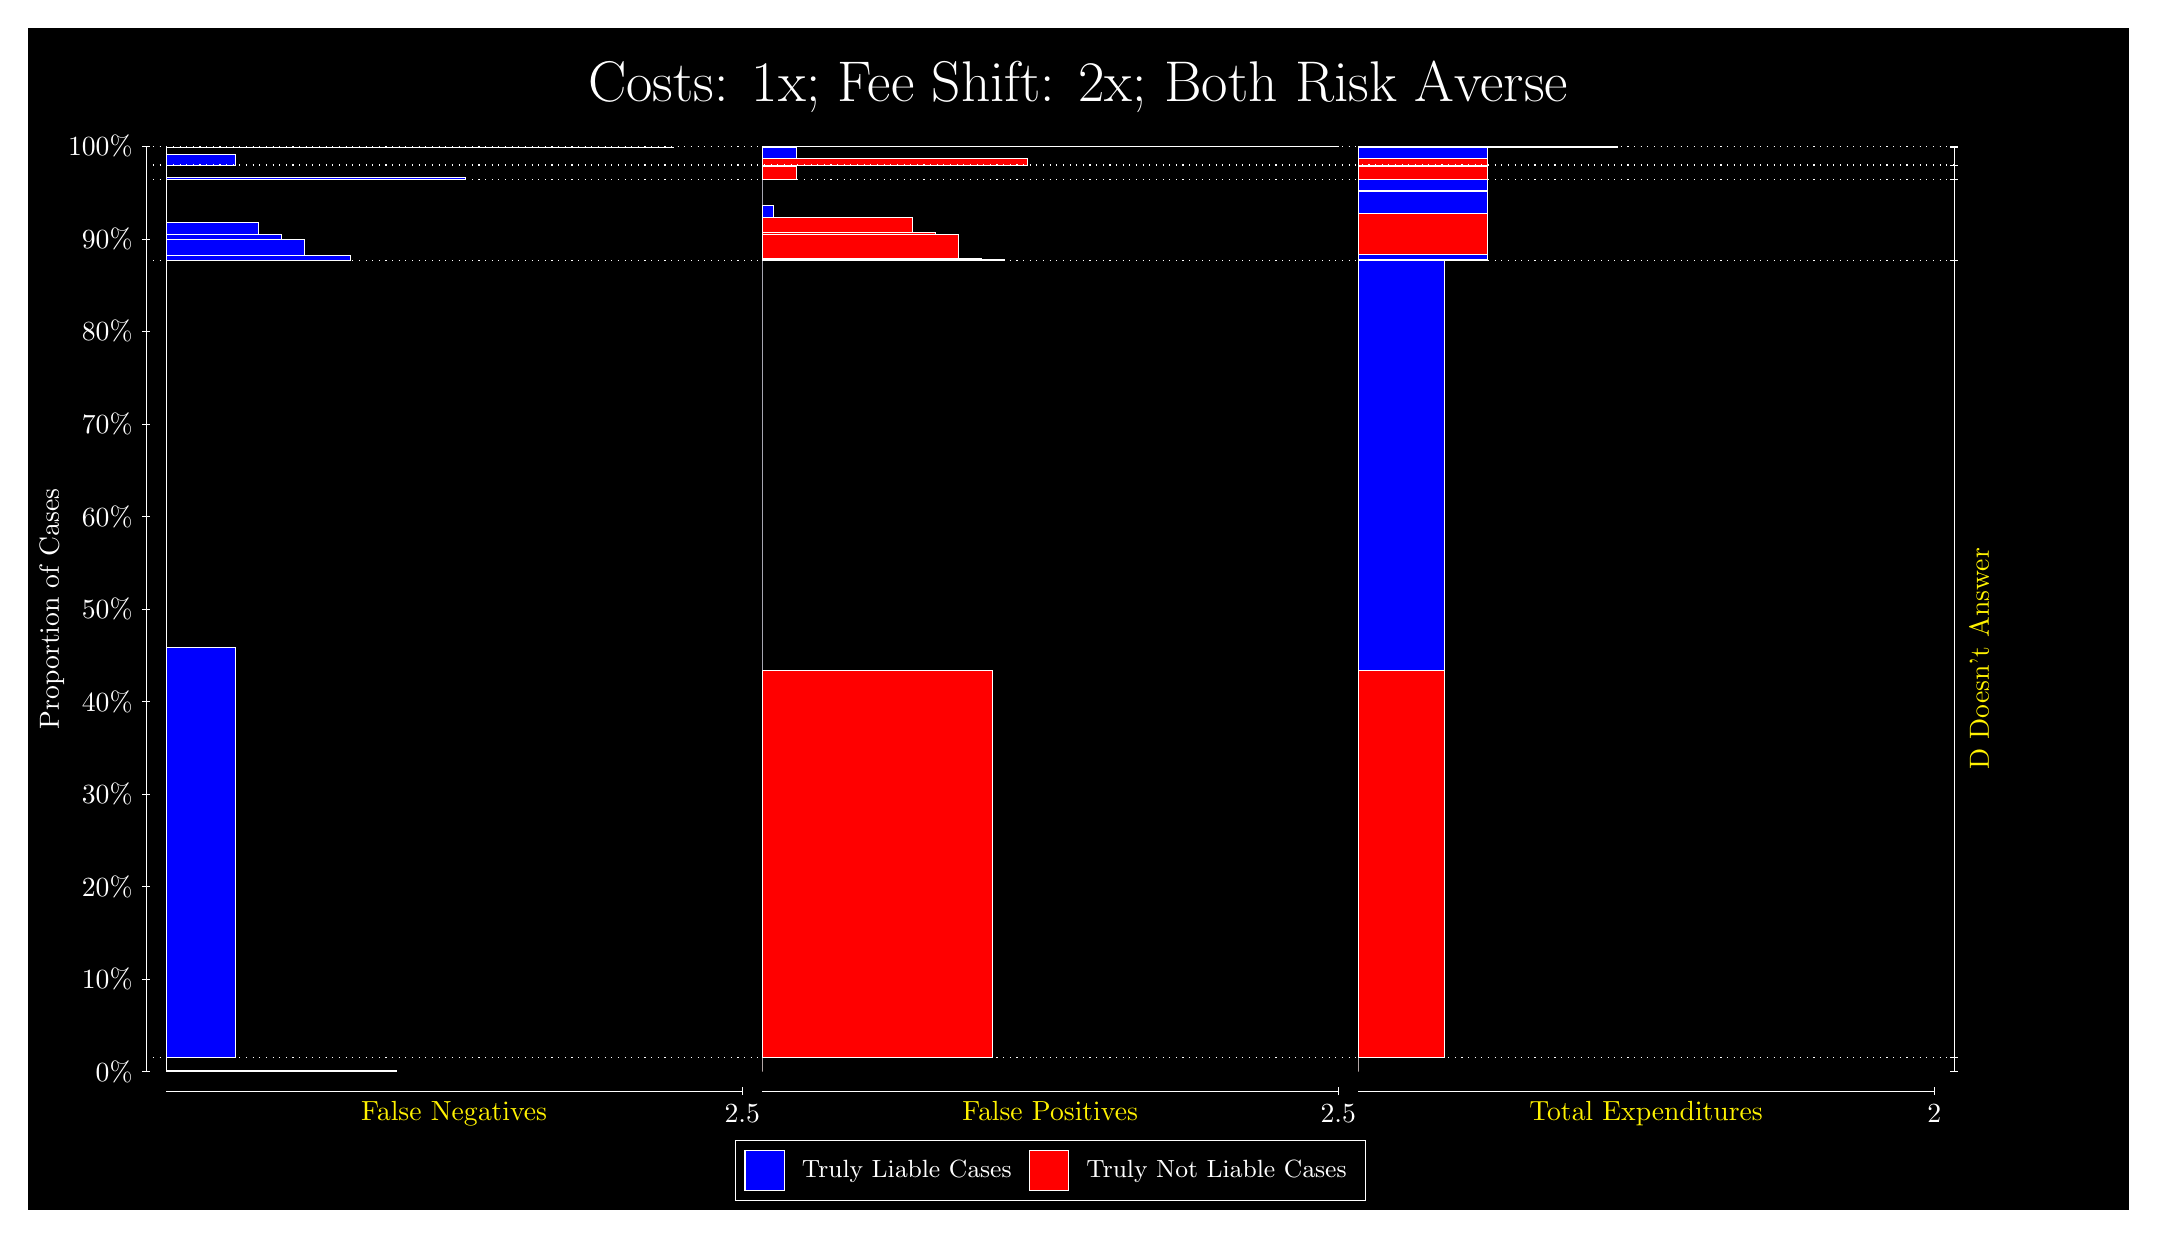
\begin{tikzpicture}
\draw[fill=black] (0,0) rectangle (26.667,15);
\draw[text=white] (0,13.5) rectangle (26.667,15) node[midway] {\huge Costs: 1x; Fee Shift: 2x; Both Risk Averse};
\draw[white, very thin] (1.5,1.75) -- (1.5,13.5);
\node[rotate=90, text=white, anchor=center] at (0.3, 7.625) {Proportion of Cases};
\draw[white, very thin] (1.45,1.75) -- (1.55,1.75);
\node[text=white, anchor=east] at (1.45, 1.75) {0\%};
\draw[white, very thin] (1.45,2.925) -- (1.55,2.925);
\node[text=white, anchor=east] at (1.45, 2.925) {10\%};
\draw[white, very thin] (1.45,4.1) -- (1.55,4.1);
\node[text=white, anchor=east] at (1.45, 4.1) {20\%};
\draw[white, very thin] (1.45,5.275) -- (1.55,5.275);
\node[text=white, anchor=east] at (1.45, 5.275) {30\%};
\draw[white, very thin] (1.45,6.45) -- (1.55,6.45);
\node[text=white, anchor=east] at (1.45, 6.45) {40\%};
\draw[white, very thin] (1.45,7.625) -- (1.55,7.625);
\node[text=white, anchor=east] at (1.45, 7.625) {50\%};
\draw[white, very thin] (1.45,8.8) -- (1.55,8.8);
\node[text=white, anchor=east] at (1.45, 8.8) {60\%};
\draw[white, very thin] (1.45,9.975) -- (1.55,9.975);
\node[text=white, anchor=east] at (1.45, 9.975) {70\%};
\draw[white, very thin] (1.45,11.15) -- (1.55,11.15);
\node[text=white, anchor=east] at (1.45, 11.15) {80\%};
\draw[white, very thin] (1.45,12.325) -- (1.55,12.325);
\node[text=white, anchor=east] at (1.45, 12.325) {90\%};
\draw[white, very thin] (1.45,13.5) -- (1.55,13.5);
\node[text=white, anchor=east] at (1.45, 13.5) {100\%};

\draw[white, very thin] (24.457,1.75) -- (24.457,13.5);
\draw[white, very thin] (24.407,1.75) -- (24.507,1.75);
\node[anchor=west] at (24.407, 1.75) {};
\draw[white, very thin] (24.407,1.9273) -- (24.507,1.9273);
\node[anchor=west] at (24.407, 1.9273) {};
\draw[white, very thin] (24.407,12.052) -- (24.507,12.052);
\node[anchor=west] at (24.407, 12.052) {};
\draw[white, very thin] (24.407,13.084) -- (24.507,13.084);
\node[anchor=west] at (24.407, 13.084) {};
\draw[white, very thin] (24.407,13.263) -- (24.507,13.263);
\node[anchor=west] at (24.407, 13.263) {};
\draw[white, very thin] (24.407,13.493) -- (24.507,13.493);
\node[anchor=west] at (24.407, 13.493) {};
\draw[white, very thin] (24.407,13.498) -- (24.507,13.498);
\node[anchor=west] at (24.407, 13.498) {};
\draw[white, very thin] (24.407,13.5) -- (24.507,13.5);
\node[anchor=west] at (24.407, 13.5) {};

\draw[white, very thin, fill=blue] (1.75,1.75) rectangle (4.6775,1.7687);
\draw[white, very thin, fill=red] (1.75,1.7687) rectangle (1.75,1.9273);
\draw[white, very thin, fill=blue] (1.75,1.9273) rectangle (2.6283,7.1396);
\draw[white, very thin, fill=red] (1.75,7.1396) rectangle (1.75,12.052);
\draw[white, very thin, fill=blue] (1.75,12.052) rectangle (4.092,12.112);
\draw[white, very thin, fill=blue] (1.75,12.112) rectangle (3.7993,12.115);
\draw[white, very thin, fill=blue] (1.75,12.115) rectangle (3.5065,12.324);
\draw[white, very thin, fill=blue] (1.75,12.324) rectangle (3.2138,12.389);
\draw[white, very thin, fill=blue] (1.75,12.389) rectangle (2.921,12.533);
\draw[white, very thin, fill=red] (1.75,12.533) rectangle (1.75,13.084);
\draw[white, very thin, fill=blue] (1.75,13.084) rectangle (5.5558,13.104);
\draw[white, very thin, fill=red] (1.75,13.104) rectangle (1.75,13.263);
\draw[white, very thin, fill=blue] (1.75,13.263) rectangle (2.6283,13.404);
\draw[white, very thin, fill=red] (1.75,13.404) rectangle (1.75,13.493);
\draw[white, very thin, fill=blue] (1.75,13.493) rectangle (8.1906,13.494);
\draw[white, very thin, fill=red] (1.75,13.494) rectangle (1.75,13.498);
\draw[white, very thin, fill=red] (1.75,13.498) rectangle (1.75,13.499);
\draw[white, very thin, fill=blue] (1.75,13.499) rectangle (1.75,13.5);
\draw[white, very thin, fill=red] (9.3189,1.75) rectangle (9.3189,1.9086);
\draw[white, very thin, fill=blue] (9.3189,1.9086) rectangle (9.3189,1.9273);
\draw[white, very thin, fill=red] (9.3189,1.9273) rectangle (12.246,6.84);
\draw[white, very thin, fill=blue] (9.3189,6.84) rectangle (9.3189,12.052);
\draw[white, very thin, fill=red] (9.3189,12.052) rectangle (12.393,12.07);
\draw[white, very thin, fill=red] (9.3189,12.07) rectangle (12.1,12.08);
\draw[white, very thin, fill=red] (9.3189,12.08) rectangle (11.807,12.383);
\draw[white, very thin, fill=red] (9.3189,12.383) rectangle (11.515,12.41);
\draw[white, very thin, fill=red] (9.3189,12.41) rectangle (11.222,12.604);
\draw[white, very thin, fill=blue] (9.3189,12.604) rectangle (9.4652,12.748);
\draw[white, very thin, fill=blue] (9.3189,12.748) rectangle (9.3189,13.084);
\draw[white, very thin, fill=red] (9.3189,13.084) rectangle (9.758,13.243);
\draw[white, very thin, fill=blue] (9.3189,13.243) rectangle (9.3189,13.263);
\draw[white, very thin, fill=red] (9.3189,13.263) rectangle (12.686,13.351);
\draw[white, very thin, fill=blue] (9.3189,13.351) rectangle (9.758,13.493);
\draw[white, very thin, fill=red] (9.3189,13.493) rectangle (9.3189,13.496);
\draw[white, very thin, fill=blue] (9.3189,13.496) rectangle (9.3189,13.498);
\draw[white, very thin, fill=red] (9.3189,13.498) rectangle (16.638,13.499);
\draw[white, very thin, fill=blue] (9.3189,13.499) rectangle (13.71,13.5);
\draw[white, very thin, fill=red] (16.888,1.75) rectangle (16.888,1.9086);
\draw[white, very thin, fill=blue] (16.888,1.9086) rectangle (16.888,1.9273);
\draw[white, very thin, fill=red] (16.888,1.9273) rectangle (17.986,6.84);
\draw[white, very thin, fill=blue] (16.888,6.84) rectangle (17.986,12.052);
\draw[white, very thin, fill=red] (16.888,12.052) rectangle (18.534,12.062);
\draw[white, very thin, fill=blue] (16.888,12.062) rectangle (18.534,12.127);
\draw[white, very thin, fill=red] (16.888,12.127) rectangle (18.534,12.651);
\draw[white, very thin, fill=blue] (16.888,12.651) rectangle (18.534,12.923);
\draw[white, very thin, fill=red] (16.888,12.923) rectangle (18.534,12.94);
\draw[white, very thin, fill=blue] (16.888,12.94) rectangle (18.534,13.084);
\draw[white, very thin, fill=red] (16.888,13.084) rectangle (18.534,13.243);
\draw[white, very thin, fill=blue] (16.888,13.243) rectangle (18.534,13.263);
\draw[white, very thin, fill=red] (16.888,13.263) rectangle (18.534,13.351);
\draw[white, very thin, fill=blue] (16.888,13.351) rectangle (18.534,13.493);
\draw[white, very thin, fill=red] (16.888,13.493) rectangle (20.181,13.496);
\draw[white, very thin, fill=blue] (16.888,13.496) rectangle (20.181,13.498);
\draw[white, very thin, fill=red] (16.888,13.498) rectangle (20.181,13.499);
\draw[white, very thin, fill=blue] (16.888,13.499) rectangle (20.181,13.5);
\draw[white, dotted] (1.5,1.9273) -- (24.457,1.9273);
\draw[white, dotted] (1.5,12.052) -- (24.457,12.052);
\draw[white, dotted] (1.5,13.084) -- (24.457,13.084);
\draw[white, dotted] (1.5,13.263) -- (24.457,13.263);
\draw[white, dotted] (1.5,13.493) -- (24.457,13.493);
\draw[white, dotted] (1.5,13.498) -- (24.457,13.498);
\draw[white, very thin] (1.75,1.5) -- (9.0689,1.5);
\node[text=yellow, anchor=north] at (5.4094, 1.5) {False Negatives};
\draw[white, very thin] (9.0689,1.45) -- (9.0689,1.55);
\node[text=white, anchor=north] at (9.0689, 1.45) {2.5};

\draw[white, very thin] (9.3189,1.5) -- (16.638,1.5);
\node[text=yellow, anchor=north] at (12.978, 1.5) {False Positives};
\draw[white, very thin] (16.638,1.45) -- (16.638,1.55);
\node[text=white, anchor=north] at (16.638, 1.45) {2.5};

\draw[white, very thin] (16.888,1.5) -- (24.207,1.5);
\node[text=yellow, anchor=north] at (20.547, 1.5) {Total Expenditures};
\draw[white, very thin] (24.207,1.45) -- (24.207,1.55);
\node[text=white, anchor=north] at (24.207, 1.45) {2};


\node[text=yellow, centered, rotate=90] at (24.777, 6.9898) {D Doesn't Answer};






\draw (12.978300999999998,1.5) node[draw=none] (baseCoordinate) {};
\begin{scope}[align=center]
        \matrix[scale=0.5, draw=white, below=0.5cm of baseCoordinate, nodes={draw}, column sep=0.1cm]{
            \node[rectangle, draw, minimum width=0.5cm, minimum height=0.5cm, fill=blue] {}; &
            \node[draw=none, font=\small, text=white] (B) {Truly Liable Cases}; &
            \node[rectangle, draw, minimum width=0.5cm, minimum height=0.5cm, fill=red] {}; &
            \node[draw=none, font=\small, text=white] (B) {Truly Not Liable Cases}; \\
            };
\end{scope}

\end{tikzpicture}
\end{document}